\documentclass{report}

\usepackage{graphicx}
\usepackage{algorithm}
\usepackage{array}
\usepackage{dsfont}
\usepackage{algpseudocode}
\usepackage{listings}
\usepackage{amsmath}
\usepackage{tikz}
\usepackage{pdfpages}
\usepackage{float}

\usetikzlibrary{automata, positioning, arrows}
\DeclareMathOperator{\rank}{rank}
\makeatletter
\newenvironment{sqcases}{%
  \matrix@check\sqcases\env@sqcases
}{%
  \endarray\right.%
}
\def\env@sqcases{%
  \let\@ifnextchar\new@ifnextchar
  \left\lbrack
  \def\arraystretch{1.2}%
  \array{@{}l@{\quad}l@{}}%
}
\makeatother

\usetikzlibrary{calc}


\input{/mnt/fa80f336-3342-4d78-8bfd-a43e434a2cda/Latex/preamble.tex}
\input{/mnt/fa80f336-3342-4d78-8bfd-a43e434a2cda/Latex/macros.tex}
\input{/mnt/fa80f336-3342-4d78-8bfd-a43e434a2cda/Latex/letterfonts.tex}

\title{\Huge{FU08 \-- Automata and Languages}\\Exercise 4}
\author{\huge{NGUYEN Tuan Dung}\\\huge{s1312004}}
\date{December 16, 2024}

\begin{document}

\maketitle

% Cau 1
\qs{Answer the following question}{
    For $\Sigma=\{0,1\}$, construct an NFA accepting the following language:\\
The set of all strings such that some two 0's are separated by a string whose length is $4 i$, for some $i \geq 0$.
}

\sol{\newline
$\bullet$ \textbf{State definition}:\\
We call the length of the interim string between the two 0's $n$. We want the following language to be accepted: $(0 \lor 1)^{*}~0~(0 \lor 1)^{4\mathrm{i}}~0~(0 \lor 1)^{*}$
\begin{itemize}
    \item $\mathrm{q}_{0}$: The string does not contain anything.
    \item $\mathrm{q}_{1}$: The string contains the first 0, and $n \% 4 = 0$.
    \item $\mathrm{q}_{2}$: The string contains the first 0, and $n \% 4 = 1$.
    \item $\mathrm{q}_{3}$: The string contains the first 0, and $n \% 4 = 2$. 
    \item $\mathrm{q}_{4}$: The string contains the first 0, and $n \% 4 = 3$.
    \item $\mathrm{q}_{5}$: The string contains the first 0, $n= 4i$ (or $n \% 4 = 0$), and a second 0. $\mathrm{q}_{5} \in \mathds{F}$.
\end{itemize}
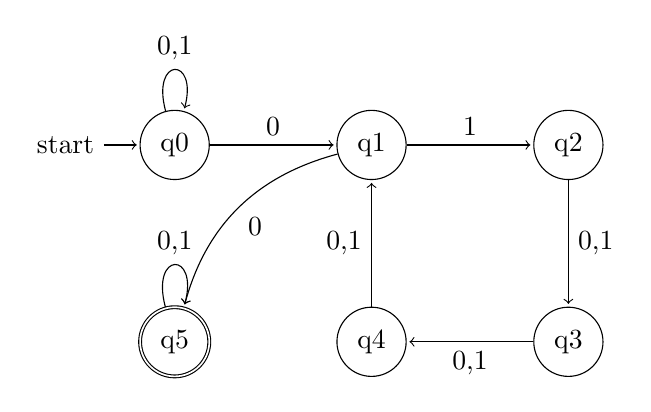
\begin{tikzpicture}[shorten >=1pt, node distance=2.5cm, on grid, auto]
    \node[state, initial] (q0)   {q0}; 
    \node[state] (q1) [right=of q0] {q1}; 
    \node[state] (q2) [right=of q1] {q2}; 
    \node[state] (q3) [below of=q2] {q3}; 
    \node[state] (q4) [below of=q1] {q4}; 
    \node[state, accepting] (q5) [below of=q0] {q5};

    \path[->]
    (q0) edge [loop above] node {0,1} (q0)
          edge node {0} (q1)
    (q1) edge node {1} (q2)
          edge [bend right] node {0} (q5)
    (q2) edge node {0,1} (q3)
    (q3) edge node {0,1} (q4)
    (q4) edge node {0,1} (q1)
    (q5) edge [loop above] node {0,1} (q5);
\end{tikzpicture}}
\newline
\pagebreak
\qs{Answer the following question}{
Construct two DFA's equivalent to the NFA's\\
(a) $M_1=\left(\{p, q, r, s\},\{0,1\}, \delta_1, p,\{s\}\right)$\\
(b) $M_2=\left(\{p, q, r, s\},\{0,1\}, \delta_2, p,\{q, s\}\right)$\\
where $\delta_1$ and $\delta_2$ are given by the following tables\\
\begin{table}[H]
      \centering
      \begin{minipage}{0.45\textwidth}
          \centering
          \begin{tabular}{|c|c|c|}
          \hline
          $\delta_1$ & 0       & 1     \\ \hline
          p & \{p,q\} & \{p\} \\ \hline
          q & \{r\}   & \{r\} \\ \hline
          r & \{s\}   & -     \\ \hline
          s & \{s\}   & \{s\} \\ \hline
          \end{tabular}
          \caption{Transition Table $\delta_1$}
      \end{minipage}
      \hfill
      \begin{minipage}{0.45\textwidth}
          \centering
          \begin{tabular}{|c|c|c|}
          \hline
          $\delta_2$ & 0       & 1       \\ \hline
          p & \{q,s\} & \{q\}   \\ \hline
          q & \{r\}   & \{q,r\} \\ \hline
          r & \{s\}   & \{p\}   \\ \hline
          s & -       & \{p\}   \\ \hline
          \end{tabular}
          \caption{Transition Table $\delta_2$}
      \end{minipage}
  \end{table}
}

\sol{\newline
\noindent a. We define a DFA $N_1 = (Q', \sum, \delta_{1}', q_{1}', \mathds{F}')$:\\
1. $Q' = \mathscr{P}(Q) = \{\emptyset, \{p\}, \{q\}, \{r\}, \{s\}, \{p,q,r,s\}, \{p, q\}, \{p, r\}, \{p, s\}, \{q, r\}, \{q, s\}, \{r, s\}, \{p,q,r\}, \{p,r,s\}, \{p,q,s\}, \{q,r,s\} \}$.\\
2. $\sum = \{ 0,1 \}$.\\
3. $q_{1}' = \{ p \}$.\\
4. $\mathds{F}' = \{ \{s\}, \{p,q,r,s\}, \{p,s\}, \{q,s\}, \{r,s\}, \{p,r,s\}, \{p,q,s\}, \{q,r,s\} \}$.\\
Since we know that $\delta_{1}'(R,a) = \{ q \in Q | q \in \delta(r,a) \mathrm{~for~} r \in R \}$. Hence, we obtain the following state transitions.\\
\newline
\begin{minipage}[t]{0.5\textwidth}
      \textbf{for a = 0}\newline
            $\delta_{1}'(\emptyset,0) = \emptyset$\\
            $\delta_{1}'(\{ p \},0) = \{ p, q \}$\\
            $\delta_{1}'(\{ q \},0) = \{ r \}$\\
            $\delta_{1}'(\{ r \},0) = \{ s \}$\\
            $\delta_{1}'(\{ s \},0) = \{ s \}$\\
            $\delta_{1}'(\{ p,q,r,s \},0) = \{ p, q \} \cup \{ r \} \cup \{ s \} \cup \{ s \} = \{ p,q,r,s \}$\\
            $\delta_{1}'(\{ p,q \},0) = \{ p, q \} \cup \{ r \} = \{ p,q,r \}$\\
            $\delta_{1}'(\{ p,r \},0) = \{ p, q \} \cup \{ s \} = \{ p,q,s \}$\\
            $\delta_{1}'(\{ p,s \},0) = \{ p, q \} \cup \{ s \} = \{ p,q,s \}$\\
            $\delta_{1}'(\{ q,r \},0) = \{ r \} \cup \{ s \} = \{ r,s \}$\\
            $\delta_{1}'(\{ q,s \},0) = \{ r \} \cup \{ s \} = \{ r,s \}$\\
            $\delta_{1}'(\{ r,s \},0) = \{ s \} \cup \{ s \} = \{ s \}$\\
            $\delta_{1}'(\{ p,q,r \},0) = \{ p,q \} \cup \{ r \} \cup \{ s \} = \{ p,q,r,s \}$\\
            $\delta_{1}'(\{ p,r,s \},0) = \{ p,q \} \cup \{ s \} \cup \{ s \} = \{ p,q,s \}$\\
            $\delta_{1}'(\{ p,q,s \},0) = \{ p,q \} \cup \{ r \} \cup \{ s \} = \{ p,q,r,s \}$\\
            $\delta_{1}'(\{ q,r,s \},0) = \{ r \} \cup \{ s \} \cup \{ s \} = \{ r,s \}$\\
\end{minipage}%
\hfill
\begin{minipage}[t]{0.48\textwidth}
      \textbf{for a = 1}\newline
            $\delta_{1}'(\emptyset,1) = \emptyset$\\
            $\delta_{1}'(\{ p \},1) = \{ p \}$\\
            $\delta_{1}'(\{ q \},1) = \{ r \}$\\
            $\delta_{1}'(\{ r \},1) = \emptyset$\\
            $\delta_{1}'(\{ s \},1) = \{ s \}$\\
            $\delta_{1}'(\{ p,q,r,s \},1) = \{ p \} \cup \{ r \} \cup \{ s \} \cup \emptyset = \{ p,r,s \}$\\
            $\delta_{1}'(\{ p,q \},1) = \{ p \} \cup \{ r \} = \{ p,r \}$\\
            $\delta_{1}'(\{ p,r \},1) = \{ p \} \cup \emptyset = \{ p \}$\\
            $\delta_{1}'(\{ p,s \},1) = \{ p \} \cup \{ s \} = \{ p,s \}$\\
            $\delta_{1}'(\{ q,r \},1) = \{ r \} \cup \emptyset = \{ r \}$\\
            $\delta_{1}'(\{ q,s \},1) = \{ r \} \cup \{ s \} = \{ r,s \}$\\
            $\delta_{1}'(\{ r,s \},1) = \emptyset \cup \{ s \} = \{ s \}$\\
            $\delta_{1}'(\{ p,q,r \},1) = \{ p \} \cup \{ r \} \cup \emptyset = \{ p,r \}$\\
            $\delta_{1}'(\{ p,r,s \},1) = \{ p \} \cup \{ s \} \cup \emptyset = \{ p,s \}$\\
            $\delta_{1}'(\{ p,q,s \},1) = \{ p \} \cup \{ r \} \cup \{ s \} = \{ p,r,s \}$\\
            $\delta_{1}'(\{ q,r,s \},1) = \{ r \} \cup \emptyset \cup \{ s \} = \{ r,s \}$\\
\end{minipage}
Now, we construct the state transition table. (next page)
\pagebreak

\noindent \textbf{State transition table}
\newline
\[
\begin{array}{|c|c|c|}
\hline
\delta_{1}' & 0 & 1 \\ \hline
\{ p \}      & \{ p, q \}        & \{ p \}           \\ \hline
\{ q \}      & \{ r \}           & \{ r \}           \\ \hline
\{ r \}      & \{ s \}           & \emptyset         \\ \hline
\{ s \}      & \{ s \}           & \{ s \}           \\ \hline
\{ p,q \}    & \{ p,q,r \}       & \{ p,r \}         \\ \hline
\{ p,r \}    & \{ p,q,s \}       & \{ p \}           \\ \hline
\{ p,s \}    & \{ p,q,s \}       & \{ p,s \}         \\ \hline
\{ q,r \}    & \{ r,s \}         & \{ r \}           \\ \hline
\{ q,s \}    & \{ r,s \}         & \{ r,s \}         \\ \hline
\{ r,s \}    & \{ s \}           & \{ s \}           \\ \hline
\{ p,q,r \}  & \{ p,q,r,s \}     & \{ p,r \}         \\ \hline
\{ p,r,s \}  & \{ p,q,s \}       & \{ p,s \}         \\ \hline
\{ p,q,s \}  & \{ p,q,r,s \}     & \{ p,r,s \}       \\ \hline
\{ q,r,s \}  & \{ r,s \}         & \{ r,s \}         \\ \hline
\{ p,q,r,s \}& \{ p,q,r,s \}     & \{ p,r,s \}       \\ \hline
\end{array}
\]
Now, we construct a DFA for this state transition table.
\newline
$\bullet$ \textbf{with $p$}\\
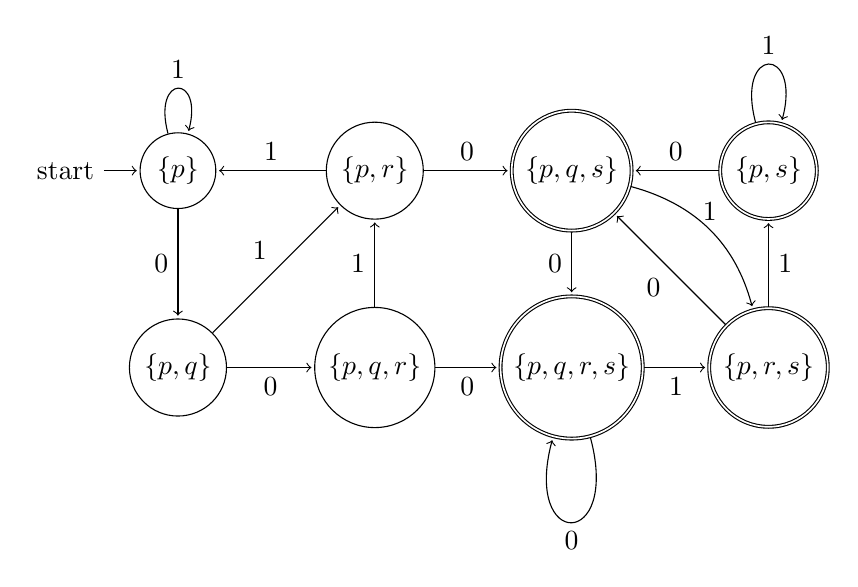
\begin{tikzpicture}[shorten >=1pt, node distance=2.5cm, on grid, auto][h]
  \node[state, initial] (p)   {$\{ p \}$}; 
  \node[state] (pr) [right=of p] {$\{ p,r \}$}; 
  \node[state, accepting] (pqs) [right=of pr] {$\{ p,q,s \}$}; 
  \node[state, accepting] (ps) [right=of pqs] {$\{ p,s \}$}; 
  \node[state] (pq) [below of=p] {$\{ p,q \}$};
  \node[state] (pqr) [below of=pr] {$\{ p,q,r \}$};
  \node[state, accepting] (pqrs) [below of=pqs] {$\{ p,q,r,s \}$};
  \node[state, accepting] (prs) [below of=ps] {$\{ p,r,s \}$};

  \path[->]
  (p) edge node[left] {0} (pq)
    (p) edge [loop above] node {1} (p)
  (pq) edge node[below] {0} (pqr)
    (pq) edge node {1} (pr)
  (pr) edge node {0} (pqs)
    (pr) edge node[above] {1} (p)
  (ps) edge node[above] {0} (pqs)
    (ps) edge [loop above] node {1} (ps)
  (pqr) edge node[below] {0} (pqrs)
    (pqr) edge node {1} (pr)
  (pqrs) edge [loop below] node {0} (pqrs)
    (pqrs) edge node[below] {1} (prs)
  (prs) edge node {0} (pqs)
    (prs) edge node[right] {1} (ps)
  (pqs) edge node[left] {0} (pqrs)
    (pqs) edge [bend left] node[above] {1} (prs);

\end{tikzpicture}
\newline
$\bullet$ \textbf{without $p$}\\
\newline
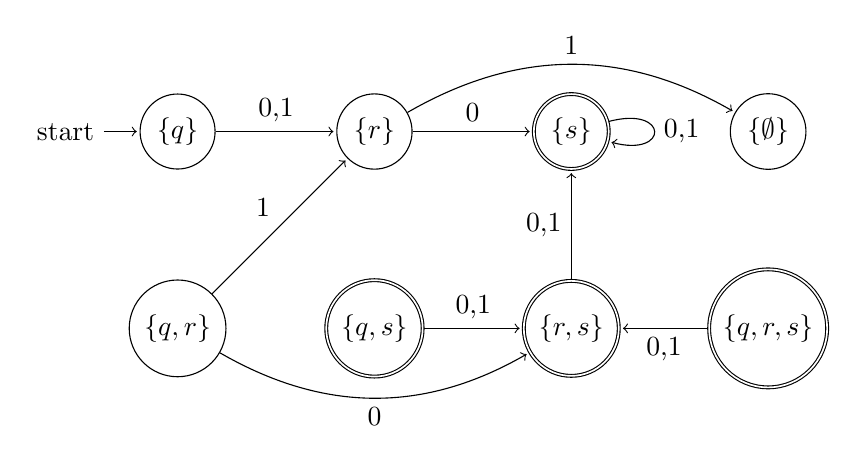
\begin{tikzpicture}[shorten >=1pt, node distance=2.5cm, on grid, auto][h]
  \node[state, initial] (q)   {$\{ q \}$}; 
  \node[state] (r) [right=of q] {$\{ r \}$}; 
  \node[state, accepting] (s) [right=of r] {$\{ s \}$}; 
  \node[state] (empty) [right=of s] {$\{ \emptyset \}$}; 
  \node[state] (qr) [below of=q] {$\{ q,r \}$};
  \node[state, accepting] (qs) [below of=r] {$\{ q,s \}$};
  \node[state, accepting] (rs) [below of=s] {$\{ r,s \}$};
  \node[state, accepting] (qrs) [below of=empty] {$\{ q,r,s \}$};

  \path[->]
  (q) edge node {0,1} (r)
  (r) edge node {0} (s)
    (r) edge[above, bend left] node {1} (empty)
  (s) edge [loop right] node {0,1} (s)
  (qr) edge [bend right] node[below] {0} (rs)
    (qr) edge node {1} (r)
  (qs) edge node {0,1} (rs)
  (rs) edge node {0,1} (s)
  (qrs) edge node {0,1} (rs);
\end{tikzpicture}
\pagebreak

\noindent b. We define a DFA $N_2 = (Q', \sum, \delta'_{2}, q_{2}', \mathds{F}')$:\\
1. $Q' = \mathscr{P}(Q) = \{\emptyset, \{p\}, \{q\}, \{r\}, \{s\}, \{p,q,r,s\}, \{p, q\}, \{p, r\}, \{p, s\}, \{q, r\}, \{q, s\}, \{r, s\}, \{p,q,r\}, \{p,r,s\}, \{p,q,s\}, \{q,r,s\} \}$.\\
2. $\sum = \{ 0,1 \}$.\\
3. $q_{2}' = \{ p \}$.\\
4. $\mathds{F}' = \{ \{ p,q,r,s \} , \{ q,s \}, \{ p,q,s \}, \{ q,r,s \}, \{ q \}, \{ s \}, \{ p,q \}, \{ p,s \}, \{ q,r \}, \{ r,s \}, \{ p,q,r \}, \{ p,r,s \} \}$.\\
Since we know that $\delta_{2}'(R,a) = \{ q \in Q | q \in \delta(r,a) \mathrm{~for~} r \in R \}$. Hence, we obtain the following state transitions.\\
\newline
\begin{minipage}[t]{0.5\textwidth}
      \textbf{for a = 0}\newline
            $\delta_{2}'(\emptyset,0) = \emptyset$\\
            $\delta_{2}'(\{ p \},0) = \{ q, s \}$\\
            $\delta_{2}'(\{ q \},0) = \{ r \}$\\
            $\delta_{2}'(\{ r \},0) = \{ s \}$\\
            $\delta_{2}'(\{ s \},0) = \{ \emptyset \}$\\
            $\delta_{2}'(\{ p,q,r,s \},0) = \{ q, s \} \cup \{ r \} \cup \{ s \} \cup \emptyset = \{ q,r,s \}$\\
            $\delta_{2}'(\{ p,q \},0) = \{ q,s \} \cup \{ r \} = \{ q,r,s \}$\\
            $\delta_{2}'(\{ p,r \},0) = \{ q,s \} \cup \{ s \} = \{ q,s \}$\\
            $\delta_{2}'(\{ p,s \},0) = \{ q,s \} \cup \emptyset = \{ q,s \}$\\
            $\delta_{2}'(\{ q,r \},0) = \{ r \} \cup \{ s \} = \{ r,s \}$\\
            $\delta_{2}'(\{ q,s \},0) = \{ r \} \cup \emptyset = \{ r \}$\\
            $\delta_{2}'(\{ r,s \},0) = \{ s \} \cup \emptyset = \{ s \}$\\
            $\delta_{2}'(\{ p,q,r \},0) = \{ q,s \} \cup \{ r \} \cup \{ s \} = \{ q,r,s \}$\\
            $\delta_{2}'(\{ p,r,s \},0) = \{ q,s \} \cup \{ s \} \cup \emptyset = \{ q,s \}$\\
            $\delta_{2}'(\{ p,q,s \},0) = \{ q,s \} \cup \{ r \} \cup \emptyset = \{ q,r,s \}$\\
            $\delta_{2}'(\{ q,r,s \},0) = \{ r \} \cup \{ s \} \cup \emptyset = \{ r,s \}$\\
\end{minipage}%
\hfill
\begin{minipage}[t]{0.48\textwidth}
      \textbf{for a = 1}\newline
            $\delta_{2}'(\emptyset,1) = \emptyset$\\
            $\delta_{2}'(\{ p \},1) = \{ q \}$\\
            $\delta_{2}'(\{ q \},1) = \{ q,r \}$\\
            $\delta_{2}'(\{ r \},1) = \{ p \}$\\
            $\delta_{2}'(\{ s \},1) = \{ p \}$\\
            $\delta_{2}'(\{ p,q,r,s \},1) = \{ q \} \cup \{ q,r \} \cup \{ p \} \cup \{ p \} = \{ p,q,r \}$\\
            $\delta_{2}'(\{ p,q \},1) = \{ q \} \cup \{ q,r \} = \{ q,r \}$\\
            $\delta_{2}'(\{ p,r \},1) = \{ q \} \cup \{ p \} = \{ p,q \}$\\
            $\delta_{2}'(\{ p,s \},1) = \{ q \} \cup \{ p \} = \{ p,q \}$\\
            $\delta_{2}'(\{ q,r \},1) = \{ q,r \} \cup \{ p \} = \{ p,q,r \}$\\
            $\delta_{2}'(\{ q,s \},1) = \{ q,r \} \cup \{ p \} = \{ p,q,r \}$\\
            $\delta_{2}'(\{ r,s \},1) = \{ p \} \cup \{ p \} = \{ p \}$\\
            $\delta_{2}'(\{ p,q,r \},1) = \{ q \} \cup \{ q,r \} \cup \{ p \} = \{ p,q,r \}$\\
            $\delta_{2}'(\{ p,r,s \},1) = \{ q \} \cup \{ p \} \cup \{ p \} = \{ p,q \}$\\
            $\delta_{2}'(\{ p,q,s \},1) = \{ q \} \cup \{ q,r \} \cup \{ p \} = \{ p,q,r \}$\\
            $\delta_{2}'(\{ q,r,s \},1) = \{ q,r \} \cup \{ p \} \cup \{ p \} = \{ p,q,r \}$\\
\end{minipage}
Now, we construct the state transition table.\\
$\bullet$ \textbf{State transition table} \newline
\begin{center}\
  \begin{tabular}{|c|c|c|}
    \hline
    \textbf{$\delta_{2}'$}        & 0 & 1 \\ \hline
    $\{ p \}$             & $\{ q, s \}$           & $\{ q \}$              \\ \hline
    $\{ q \}$             & $\{ r \}$              & $\{ q, r \}$           \\ \hline
    $\{ r \}$             & $\{ s \}$              & $\{ p \}$              \\ \hline
    $\{ s \}$             & $\emptyset$            & $\{ p \}$              \\ \hline
    $\{ p,q \}$           & $\{ q, r, s \}$        & $\{ q, r \}$           \\ \hline
    $\{ p,r \}$           & $\{ q, s \}$           & $\{ p, q \}$           \\ \hline
    $\{ p,s \}$           & $\{ q, s \}$           & $\{ p, q \}$           \\ \hline
    $\{ q,r \}$           & $\{ r, s \}$           & $\{ p, q, r \}$        \\ \hline
    $\{ q,s \}$           & $\{ r \}$              & $\{ p, q, r \}$        \\ \hline
    $\{ r,s \}$           & $\{ s \}$              & $\{ p \}$              \\ \hline
    $\{ p,q,r \}$         & $\{ q, r, s \}$        & $\{ p, q, r \}$        \\ \hline
    $\{ p,r,s \}$         & $\{ q, s \}$           & $\{ p,q \}$           \\ \hline
    $\{ p,q,s \}$         & $\{ q, r, s \}$        & $\{ p, q, r \}$        \\ \hline
    $\{ q,r,s \}$         & $\{ r, s \}$           & $\{ p, q, r \}$        \\ \hline
    $\{ p,q,r,s \}$       & $\{ q, r, s \}$        & $\{ p, q, r \}$        \\ \hline
  \end{tabular}
\end{center}
Now, we construct a DFA for this transition table. (next page)
\pagebreak

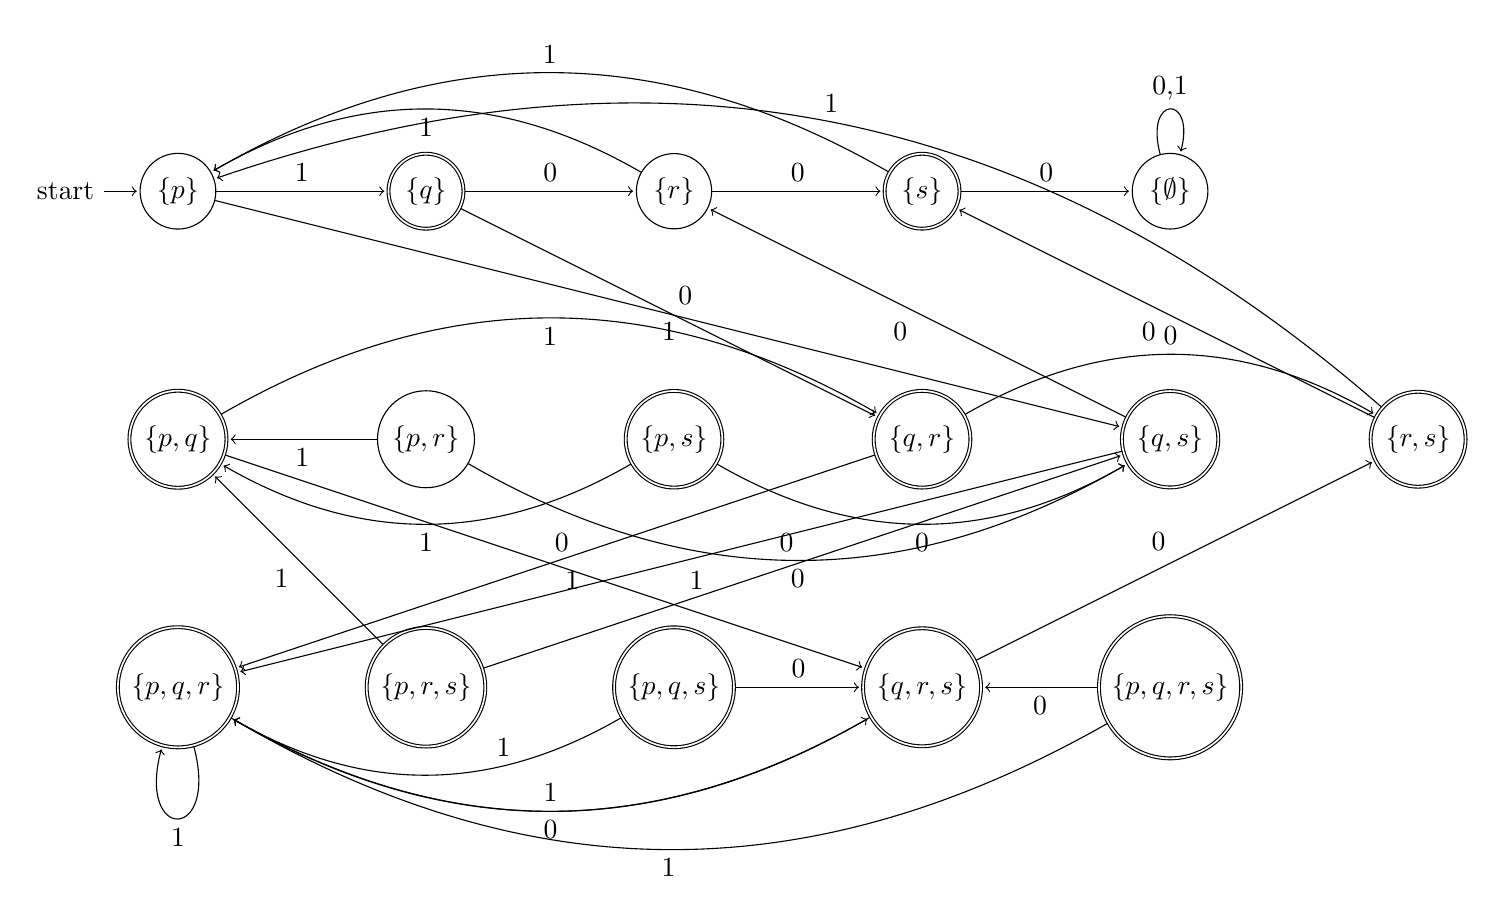
\begin{tikzpicture}[shorten >=1pt, node distance=3.15cm, on grid, auto][h]
  \node[state, initial] (p) {$\{ p \}$};
  \node[state, accepting] (q) [right=of p] {$\{ q \}$};
  \node[state] (r) [right=of q] {$\{ r \}$};
  \node[state, accepting] (s) [right=of r] {$\{ s \}$};
  \node[state] (empty) [right=of s] {$\{ \emptyset \}$};
  \node[state, accepting] (pq) [below of=p] {$\{ p,q \}$};
  \node[state] (pr) [right=of pq] {$\{ p,r \}$};
  \node[state, accepting] (ps) [right=of pr] {$\{ p,s \}$};
  \node[state, accepting] (qr) [right=of ps] {$\{ q,r \}$};
  \node[state, accepting] (qs) [right=of qr] {$\{ q,s \}$};
  \node[state, accepting] (rs) [right=of qs] {$\{ r,s \}$};
  \node[state, accepting] (pqr) [below of=pq] {$\{ p,q,r \}$};
  \node[state, accepting] (prs) [right=of pqr] {$\{ p,r,s \}$};
  \node[state, accepting] (pqs) [right=of prs] {$\{ p,q,s \}$};
  \node[state, accepting] (qrs) [right=of pqs] {$\{ q,r,s \}$};
  \node[state, accepting] (pqrs) [right=of qrs] {$\{ p,q,r,s \}$};

  \path[->]
  (p) edge node {0} (qs)
    (p) edge node {1} (q)
  (q) edge node {0} (r)
    (q) edge node[below] {1} (qr)
  (r) edge node {0} (s)
    (r) edge[above, bend right] node[below] {1} (p)
  (s) edge node {0} (empty)
    (s) edge[above, bend right] node {1} (p)
  (pq) edge node {0} (qrs)
    (pq) edge[above, bend left] node[below] {1} (qr)
  (pr) edge[below, bend right] node {0} (qs)
    (pr) edge node {1} (pq)
  (ps) edge[below, bend right] node {0} (qs)
    (ps) edge[below, bend left] node {1} (pq)
  (qr) edge[above, bend left] node {0} (rs)
    (qr) edge node {1} (pqr)
  (qs) edge node {0} (r)
    (qs) edge node {1} (pqr)
  (rs) edge node {0} (s)
    (rs) edge[above, bend right] node {1} (p)
  (pqr) edge[below, bend right] node {0} (qrs)
    (pqr) edge[loop below] node {1} (pqr)
  (prs) edge node {0} (qs)
    (prs) edge node {1} (pq)
  (pqs) edge node {0} (qrs)
    (pqs) edge[below, bend left] node[above, pos = .3] {1} (pqr)
  (qrs) edge node {0} (rs)
    (qrs) edge[below, bend left] node[above] {1} (pqr)
  (pqrs) edge node {0} (qrs)
    (pqrs) edge[below, bend left] node {1} (pqr)
  (empty) edge[loop above] node {0,1} (empty);
\end{tikzpicture}
Since the graph is messy and I could not find a way to draw it efficiently. Please refer to the state transition table to check.\newline
$\bullet$ \textbf{State transition table} \newline
\begin{center}\
  \begin{tabular}{|c|c|c|}
    \hline
    \textbf{$\delta_{2}'$}        & 0 & 1 \\ \hline
    $\{ p \}$             & $\{ q, s \}$           & $\{ q \}$              \\ \hline
    $\{ q \}$             & $\{ r \}$              & $\{ q, r \}$           \\ \hline
    $\{ r \}$             & $\{ s \}$              & $\{ p \}$              \\ \hline
    $\{ s \}$             & $\emptyset$            & $\{ p \}$              \\ \hline
    $\{ p,q \}$           & $\{ q, r, s \}$        & $\{ q, r \}$           \\ \hline
    $\{ p,r \}$           & $\{ q, s \}$           & $\{ p, q \}$           \\ \hline
    $\{ p,s \}$           & $\{ q, s \}$           & $\{ p, q \}$           \\ \hline
    $\{ q,r \}$           & $\{ r, s \}$           & $\{ p, q, r \}$        \\ \hline
    $\{ q,s \}$           & $\{ r \}$              & $\{ p, q, r \}$        \\ \hline
    $\{ r,s \}$           & $\{ s \}$              & $\{ p \}$              \\ \hline
    $\{ p,q,r \}$         & $\{ q, r, s \}$        & $\{ p, q, r \}$        \\ \hline
    $\{ p,r,s \}$         & $\{ q, s \}$           & $\{ p,q \}$           \\ \hline
    $\{ p,q,s \}$         & $\{ q, r, s \}$        & $\{ p, q, r \}$        \\ \hline
    $\{ q,r,s \}$         & $\{ r, s \}$           & $\{ p, q, r \}$        \\ \hline
    $\{ p,q,r,s \}$       & $\{ q, r, s \}$        & $\{ p, q, r \}$        \\ \hline
    % \hfill
  \end{tabular}
\end{center}
}
\end{document}
